\chapter{Zabezpečení a autentizace}
%TODO hoří má panenko kurva
V této kapitole si projdeme základní autentizační protokoly a standardy.
Pro jednoduchost se zaměříme na standardy v OpenAPI ve verzi 3.0.
Autorizaci používáme pro prevenci zneužití a kontrolu nad tím kdo jak API používá a jak často.

\section{API key}
%odkaz na api key zdroj https://swagger.io/docs/specification/authentication/api-keys/
% https://www.fortinet.com/resources/cyberglossary/api-key#:~:text=API%20Keys%20Definition%20and%20Meaning,a%20white%2Dlabeled%20internal%20marketplace.
API klíč je unikátní token který umožňuje uživateli se autorizovat. Na základě tohoto klíče se přidělí oprávnění. Mohou být poslády jako query param  \texttt{GET /something?key=rea11ysecr5tApIKeY} nebo v hlavičce requestu či jako Cookie \texttt{X-KEY: rea11ysecr5tApIKeY}. API klíč by měl znát jen server a daný klient. Takováto autentizace je brána jako bezpečná pouze při použití dalších bezpečnostních prvků jako je třeba HTTPS/SSL.

\subsection{Popis API klíče}
\begin{listing}[ht]
    \inputminted[]{yaml}{resources/code/security/openapi-key.yml}
    \caption{OpenAPI 3.0 definice}
    \label{code:api_key}
\end{listing}

Nejčastější použití API klíče je hlavně pro blokování anonymních požadavků. To vyfiltruje případný škodlivý provoz na API. Dále díky jeho jednoduchosti se často používá mezi IoT zařízeními.

V tomto příkladě jsme si definovali název API key \texttt{X-API-key} který bude v headeru (\ref{code:api_key} řádek 8). Dále s tím můžeme pracovat jako s \texttt{ApiKeyAuth} a dávat jej do všech ostatních definic endpointů pokud by bylo třeba specifikovat (\ref{code:api_key} řádek 20,21). Jinak za pomocí \ref{code:api_key} řádek 11,12 aplikujeme autorizaci na všechny operace.


Můžeme mít i více API klíčů. Například pro specifikování uživatele a specifikování aplikace.

Při nevalidním nebo chybějícím klíči můžeme vrátit chybový kód 401 který značí neoprávněný přístup. Můžeme si ho definovat takto \ref{code:api_key} řádek 11-16.





\section{Json web token} %TODO cite or smthng https://jwt.io/introduction
JWT je otevřená industriální standardizovaná % \verb|\glossary{rfc7519}| TODO
metoda pro bezpečné přeposílání zpráv ve formátu JSON objektu mezi dvěma stranami.
Tyto objekty mohou být zkontrolovány a může se jim důvěřovat, protože jsou digitálně podepsány pomocí tajného klíče nebo pomocí páru veřejného a privátního klíče za pomocí RSA nebo ECDSA algoritmu.

Nejčastěji se používá pro \textbf{autorizaci} a pro \textbf{výměnu informací}. Při \textbf{autorizaci}, když se jednou uživatel přihlásí, tak každý další požadavek bude s JWT, což dovoluje uživateli přistupovat tam, kde by bez přihlášení nemohl. Single Sign On
%\verb|\ref{sso} (btw všb přihlašováky)| TODO
především využívá JWT díky malé režii a jednoduchosti použití v různých doménách. JSON web tokeny jsou taktéž dobrý způsob jak bezpečně \textbf{vyměňovat informace} mezi více stranami díky digitálním podpisům.

\subsection{Struktura}
V kompaktní zakódované formě JWT vypadá takto: \texttt{xxxxxx.yyyyyyy.zzzzzz} , kde \texttt{x} je zakódovaný header, \texttt{y} je Payload a \texttt{z} je podpis.

\begin{description}
    \item[Header] typicky se skládá ze dvou částí. Typ tokenu a podepisovací algoritmus který byl použit. Jako třeba SHA256 nebo RSA. (\ref{code:JWT_example} řádek 3)
    \item[Payload] obsahuje data o entitě a jiná další data. (\ref{code:JWT_example} řádek 9)
    \item[Signature] neboli podpis se vytvoří tak že se zkombinuje header, payload a secret a zašifruje se příslušným algoritmem. (\ref{code:JWT_example} řádek 15)
\end{description}

\begin{listing}[ht]
    \inputminted[]{json}{resources/code/security/JWT.jsonc}
    \caption{Příklad hlavičky, obsahu a podpisu v JWT} % TODO whatever nějaké cite nebo něco https://jwt.io/introduction
    \label{code:JWT_example}
\end{listing}






\section{OAuth 2.0}
Oauth 2.0 je autorizační framework který poskytuje limitovaný přístup k datům. Nahrazuje Oauth z roku 2012 a dnes se již považuje za standard pro online autorizaci. Poskytuje přístup a omezuje akce co může klientská aplikace provádět s daty, bez toho aby se sdílely přihlašovací údaje uživatele.
% TODO kdyžtak jak to vypadá ve švagrovi


\subsection{Principy}
Oauth 2.0 je autorizační ne autentizační protokol. To znamená že je určen pro získání přístupových práv ke zdrojům. Ne k ověření identity uživatele, i když ho lze i využít k ověření identity.

Používají se zde přístupové tokeny. Přístupový token je řetězec který reprezentuje oprávnění k přístupu k datům. I když Oauth 2.0 nemá nijak definovaný formát přístupového tokenu tak se nejčastěji využívá JWT (TODO glossary json web token). Taktéž tokeny mohou mít datum vypršení platnosti.

\subsection{Role}\label{sec:Oauth_roles}
%TODO nějaký text


\begin{description}
    \item[Resource owner] je uživatel, co povoluje přístup aplikace k jeho účtu. Přístup aplikace je limitován rozsahem uděleného oprávnění
    \item[Client] je aplikace (chce používat uživatel) co chce přístup k uživatelskému účtu. Tu však musí nejdříve uživatel oprávnit a oprávnění musí validováno API.
    \item[Resource server] má uložená uživatelská data a http služby co mohou poskytovat uživatelská data autentizovaným klientům. Resource server poskytuje uživatelská data a autorizační server kontroluje identitu uživatele a poskytuje token aplikaci.
    \item[Authorization server] je zodpovědný za ověření uživatelské identity a poskytuje autentizační token. Tento token je přijímán resource serverem
\end{description}

\begin{figure}[H]
    \centering
    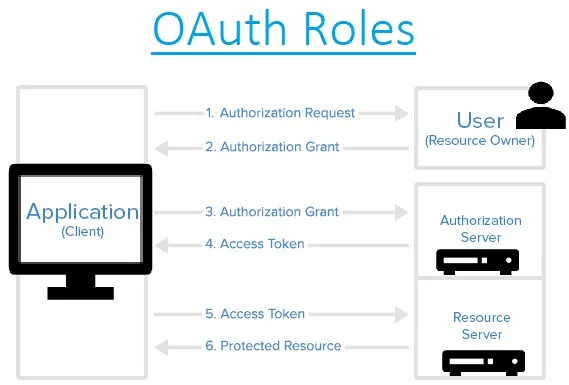
\includegraphics[width=0.7\textwidth]{figures/OAuth_abstract_flow.png}
    \caption{Abstraktní průběh protokolu}%\cite{https://medium.com/@greekykhs/ro-acd8cb4cc0f4#:~:text=OAuth%202.0%20defines%20four%20roles,Resource%20Server%20and%20Authorization%20Server.}} TODO 
    \label{fig:Oauth_roles_diagram}
\end{figure}

\subsection{Grant type: Authorization code}
Nejčastěji používaná metoda, protože je optimalizována pro stranu serveru. Autorizační server vrátí autorizační kód na jedno použití který je pak vyměněn za přístupový token. Podobné jako když se uživatelé přihlašují do webových aplikací s jejich Facebook nebo Google účtem.

\begin{figure}[ht]
    \centering
    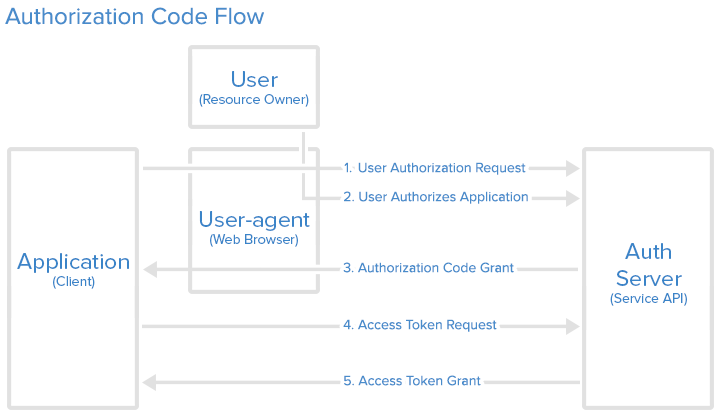
\includegraphics[width=\textwidth]{figures/OAuth_code_flow.png}
    \caption[short]{Průběh autorizace pomocí autorizačního kódu}%TODO https://www.digitalocean.com/community/tutorials/an-introduction-to-oauth-2
    \label{fig:Oauth_auth_flow}
\end{figure}


\ref{fig:Oauth_auth_flow} Nejdříve je uživateli poskytnut autorizační URL. zde se musí přihlásit do přihlašovací služby. Poté potvrdí či zamítnou aplikaci přístup k jejich účtu. Aplikace poté obdrží autorizační kód třeba přes query param %(TODO query param \verb|\ref{desc:query_param}|) 
v URL. Aplikace poté požádá o přístupový token s dalšími autentizačními detaily. A nakonec aplikace dostane přístupový token \textit{případně obnovovací token} pokud autorizace je validní.


